\chapter{Requisiti specifici}
In questo capitolo verranno illustrati le funzionalità identificate dal capitolato d'appalto \textit{GDP-Gathering Detection Platform}. 
\section{Acquisizione dati}
Il progetto preleverà dati da sorgenti esterne o simulate attraverso appositi software creati dal progettista. I dati verranno storicizzati all'interno di un database, questo sarà sviluppato usando Apache Kafka un sistema distribuito che consiste di server e client i quali comunicano tra loro attraverso un protocollo di rete performante di tipo TCP.

\section{Elaborazione Dati}
Ottenuti i dati, essi verranno elaborati attraverso librerie di sci-kit e tensorflow con il linguaggio di programmazione python
\begin{itemize}
	\item Input: i dati vengono prelevati dal server.
	\item Output: i dati elaborati vengono inviati alla pagina front-end per la visualizzazione in heat-map
	\item Processo: l'elaborazione avviene attraverso lo sviluppo di funzioni usando sci-kit learn.
\end{itemize}
\section{Visualizzazione dati}
La pagina web creata attraverso html, php e javascript permetterà la visualizzazione dei dati elaborati. I dati verranno prelevati attraverso relative query al server utilizzando il linguaggio di programmazione php.
La pagina sarà suddivisa principalmente in tre parti: 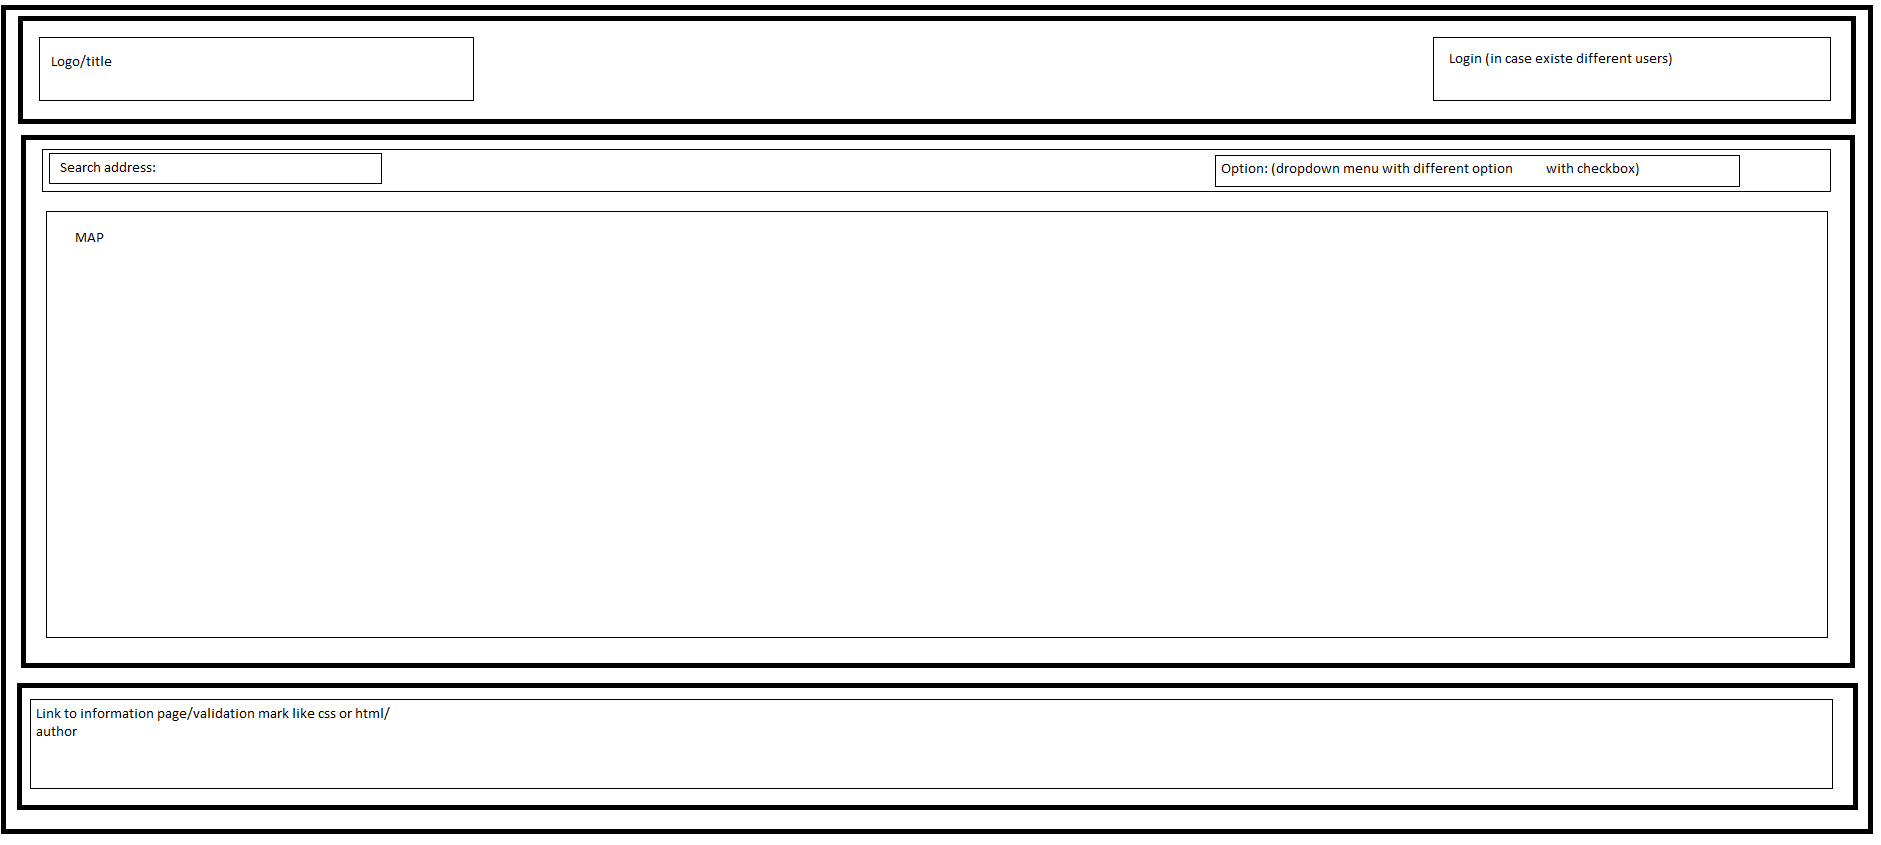
\includegraphics{../immagini/templateHtmlGDP.png}.\\
La sezione in alto individua un banner per il logo e login per gli utenti admin per effettuare modifiche alla mappa.
La sezione centrale visualizza la heat-map, una search bar per cercare il sito di assembramento che si vuole controllare e a lato di essa un menù per impostazioni di parametri aggiuntivi.\\
la sezione di footer sarà utilizzata per inserimento di informazioni sull'azienda proponente, il gruppo Jawa Druids e link per relativi ai propri siti web.